%!TEX root = ../main.tex

\section*{Summary}
\addcontentsline{toc}{section}{Summary}
\label{summary}

\subsection*{Overall: You need to trust google}
(1) a cloud provider can fake all interaction with you and therefore there should always be a level of shared-trust (also known as the matrix effect). 

\subsection*{Hardware and Virtualisation Layer: trust google}
(2) it is possible to encrypt data-storage using external keys and encrypting-decrypting in the cloud, by sending data to an external encrypting-decrypting device (HSM\footnote{\url{https://en.wikipedia.org/wiki/Hardware_security_module}}) or by using Operating System based Hard Disk encryption at the Virtual Machine Level.

(3) The AMD chip of the type EPYC promises to encrypt-decrypt data in the processing unit (CPU) and in the memory.  In the first generation of this CPU (AMD-SEV, 7001, Napels), many vulnerabilities were found that would enable other users and threat-actor to read the data. These vulnerabilities could be mitigated by actions of Google. 

This includes increased controls that the hardware is not accessed and tampered with (hardware integrity) and increased hardening of the software virtualization layer (KVM Hypervisor) that is being used. These mitigation also put all the trust at Google.

(4) In the 3rd generation CPU, the AMD-SEV-SNP CPU (7003, Milan) many of these vulnerabilities should be fixed, but due to this being a relatively new technology it is likely that in this version also new vulnerabilities will be found. Currently (2022) Google Cloud Platform does not offer the AMD-SEV-SNP CPU. 

\subsection*{Virtual Machine Layer: OK enough}
(5) On the Operating System level there are good practices to follow in making sure that another user of the system can not get access to the data (OS level encryption), here conclusion (1) is the main threat. 

\subsection*{Application Layer: OK enough}
(6) It is possible to use network encryption certificates from an external source (HSM) to communicate encrypted between applications without others (incl google) listening in. It is important to be very precise in validating the chain-of-trust\footnote{\url{ https://en.wikipedia.org/wiki/Chain_of_trust}} including the validation of the root certificate from the 
Certificate Authority\footnote{\url{https://en.wikipedia.org/wiki/Public_key_infrastructure}} (CA). 

\newpage
\subsection*{Conclusion}
Currently it is possible to decouple the compute of your data, the storage and transmission of your data from other parties except for Google as Cloud Supplier and hardware suppliers (as for example AMD). 

\begin{figure}[!ht]
    \centering
    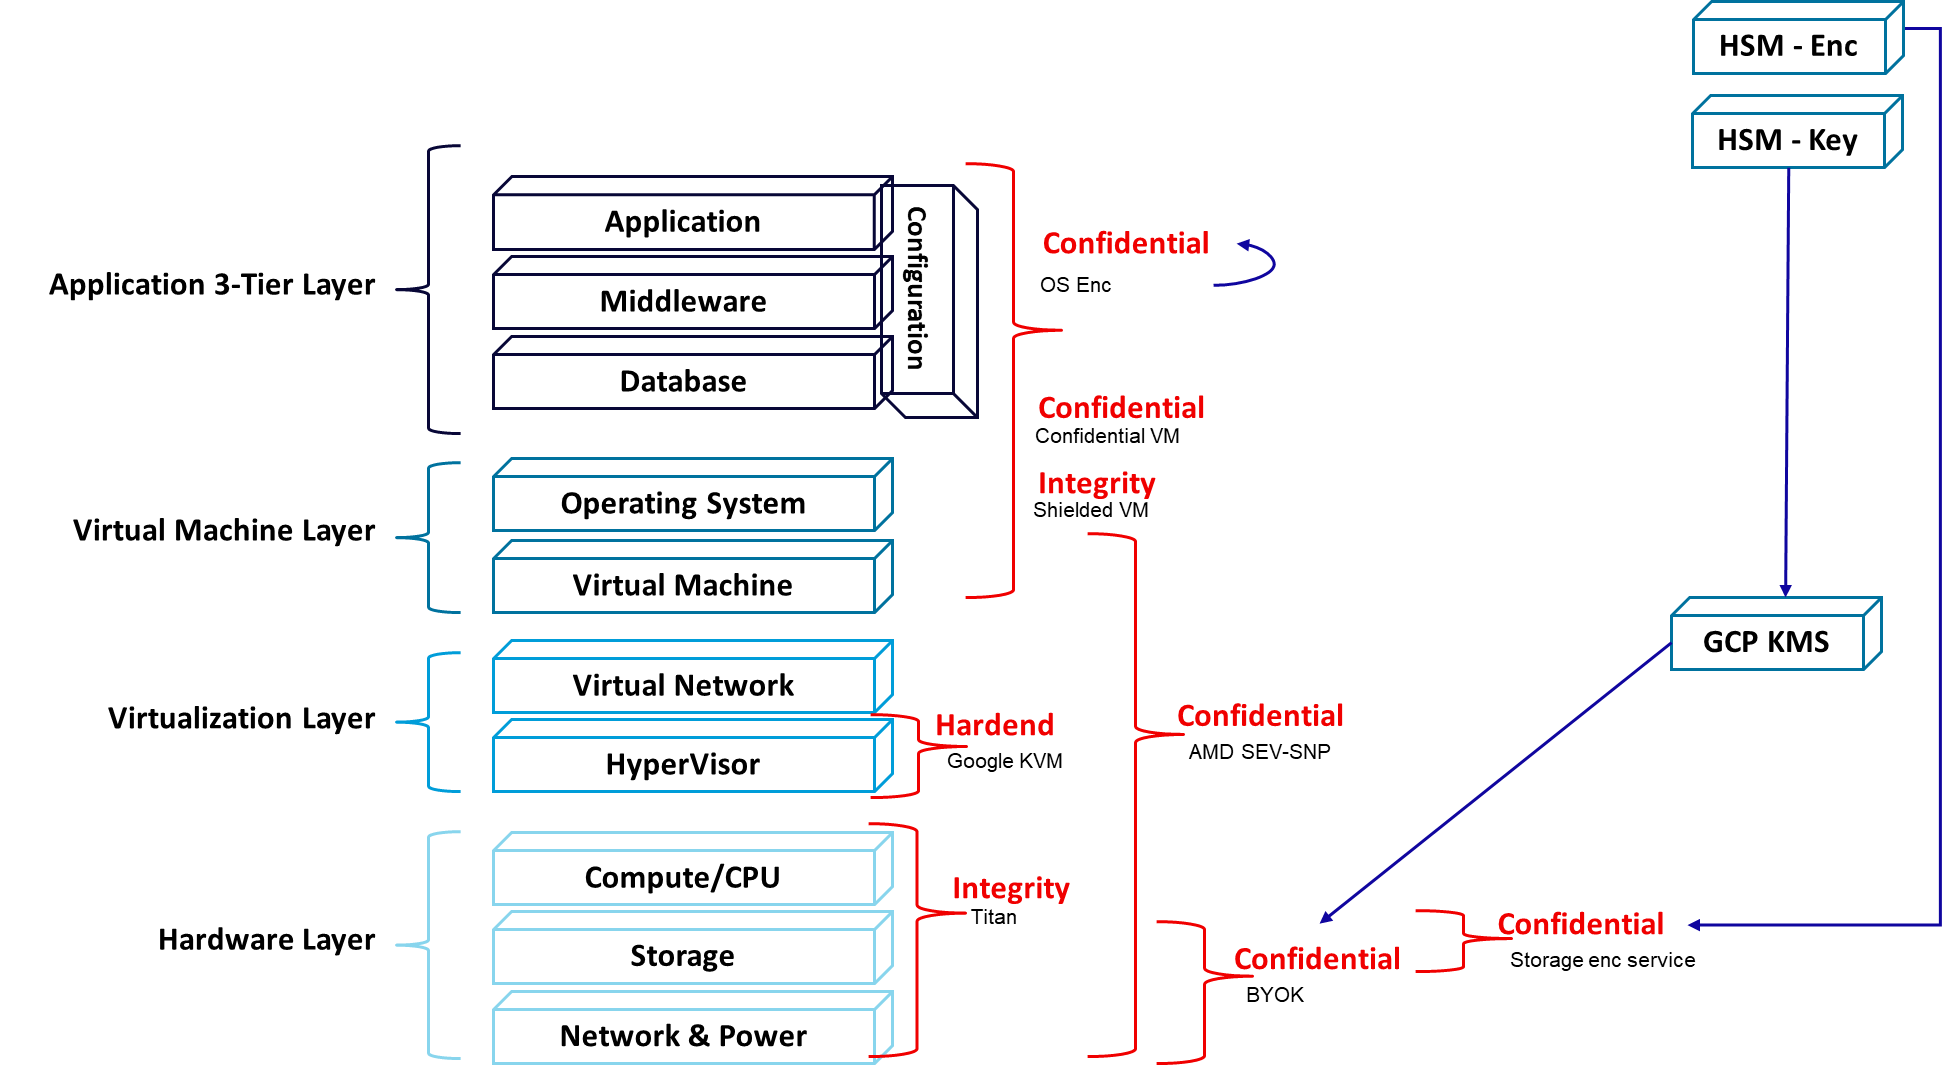
\includegraphics[width=\linewidth]{conclusion-01}
    \caption{OSI-Cloud Stack}
    \label{fig:conclusion-01}
\end{figure}

\begin{figure}[!ht]
    \centering
    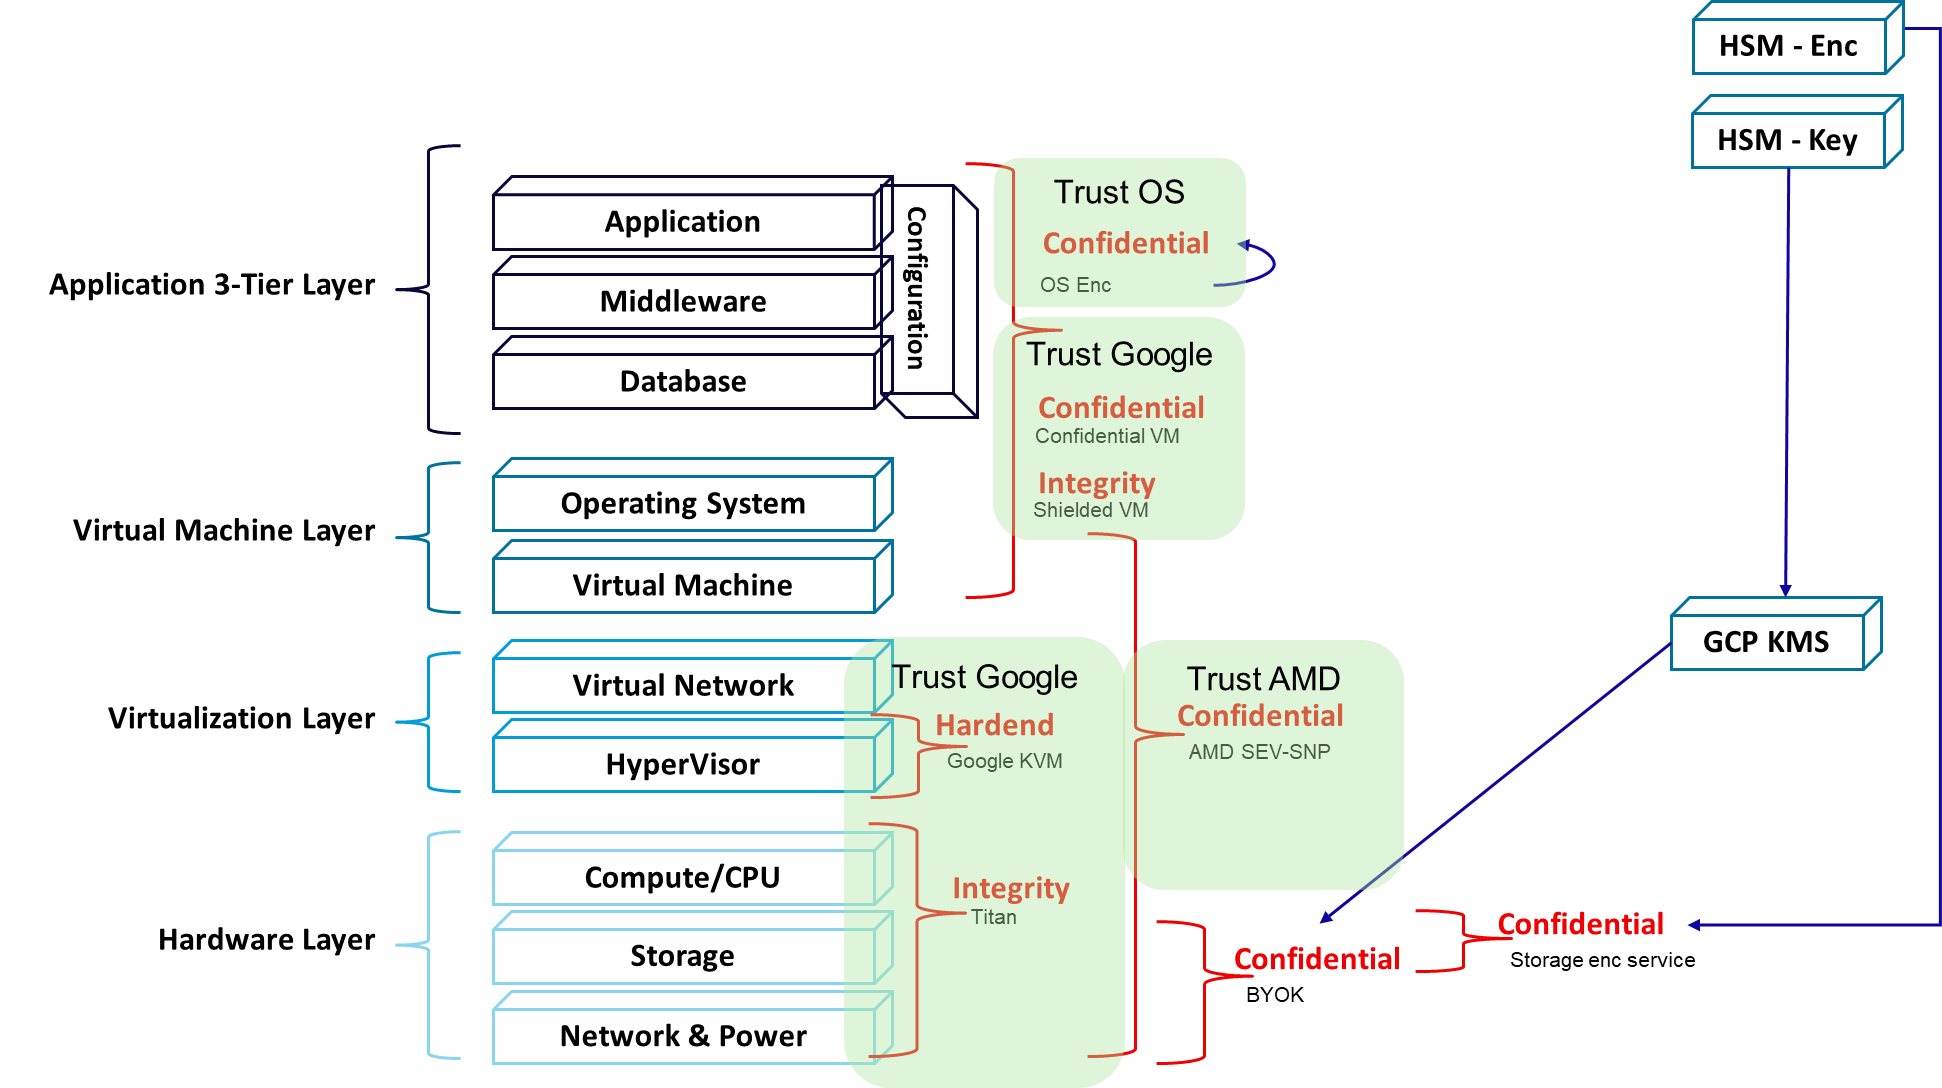
\includegraphics[width=\linewidth]{conclusion-02}
    \caption{Trust domains @OSI-Cloud Stack}
    \label{fig:conclusion-02}
\end{figure}